\apendice{Especificación de diseño}

\section{Introducción}
A lo largo de este punto veremos la especificación de diseño, donde veremos en profundidad que tipo de datos maneja y trata nuestra aplicación.

\section{Diseño de datos}
Aquí veremos qué datos se recogen, se generan y se aplican en nuestro software.

Los tipos datos de entrada que son utilizados en esta aplicación podríamos dividirlos en dos debido a su naturaleza, teniendo en cuenta que ambos son recogidos por los dispositivos de realidad virtual \cite{VR} de los que disponemos.

\subsection{Datos de Entrada}
    \begin{itemize}
        \item \textbf{Coordenadas de posición:} El tipo de datos más importante dentro de nuestro software es aquel referente a las coordenadas de posición que recoge Unity a través de nuestros controladores y las gafas de Oculus. Son coordenadas englobadas en un tipo de Unity que es un vector que tiene tres valores, ya que representan las tres dimensiones del espacio X Y Z.
        Como hemos visto previamente en este documento y en la memoria, este tipo de datos es el que nos da la posibilidad de representar correctamente nuestras manos en el espacio tridimensional, además de ser indispensable para poder enviar las instrucciones de posición necesarias a nuestro robot.
        
        Estos datos se recogen gracias a las gafas que a través de sus cámaras y sensores permite conocer en que punto de la zona establecida para usar Oculus se encuentran los controladores.
        
        Estos datos una vez recogidos, se procesan de manera que cumplan con el estándar establecido por mi previamente en búsqueda de una experiencia del usuario correcta. 
        
        \item \textbf{Datos de flexión y aducción}: Este tipo de datos es el que nos dará la posibilidad de aplicar un cierre o apertura determinado a nuestra pinza robótica. Se recogen directamente de los sensores dispuestos en el guante háptico y reflejan en un vector de tres partes los valores de pronación/supinación, flexión/extensión y adducción/abudcción de los dedos. 
        
        Los que utilizamos principalmente son los de flexión/extensión, ya que gracias a ellos podemos definir correctamente un comportamiento para la aplicación asociado a flexionar índice y pulgar simulando la pinza.
        
        Estos datos se recogen garcias al script \textit{GettingData}  y se pasan en forma de mensajes(instrucciones) para la pinza y así abrir o cerrar la pinza.
  \end{itemize}
  
\subsection{Datos Generados}
        Los datos que se generan en esta aplicación son mensajes ROS que se publican en los topics determinados, para hacer al robot cumplir con la tarea determinada. En este caso se generan dos tipos de mensajes específicos, unos referentes a la posición y rotación de la pinza y otros en relación con la apertura/cierre de la misma. 
        
        Estos mensajes se generan de manera constante ya que sus funciones se ejecutan constántemente mientras la aplicación esté funcionando. De esta manera conseguimos un resultado óptimo sin demasiado delay.

\section{Diseño arquitectónico}
En cuanto a la arquitectura dentro de este proyecto cabe destacar, que aunque el software final es una recopilación de objetos y técnicas utilizadas a lo largo del proyecto, hasta llegar a ese punto ha sido necesario del desarrollo de varias escenas para el aprendizaje y el análisis de cómo se gestionan o recogen los datos.

Cada una de esas escenas fue llevándose a cabo para cumplir pequeñas tareas y utilizando scripts que nos permitirían en un futuro, alcanzar el resultado que tenemos.

En el siguiente diagrama podemos ver la arquitectura del software final, donde cada una de las funciones o procedimientos que vemos están realizadas por scripts desarrollados:

\begin{figure}[h]
\centering
\label{Diagrama de la arquitectura del software final}
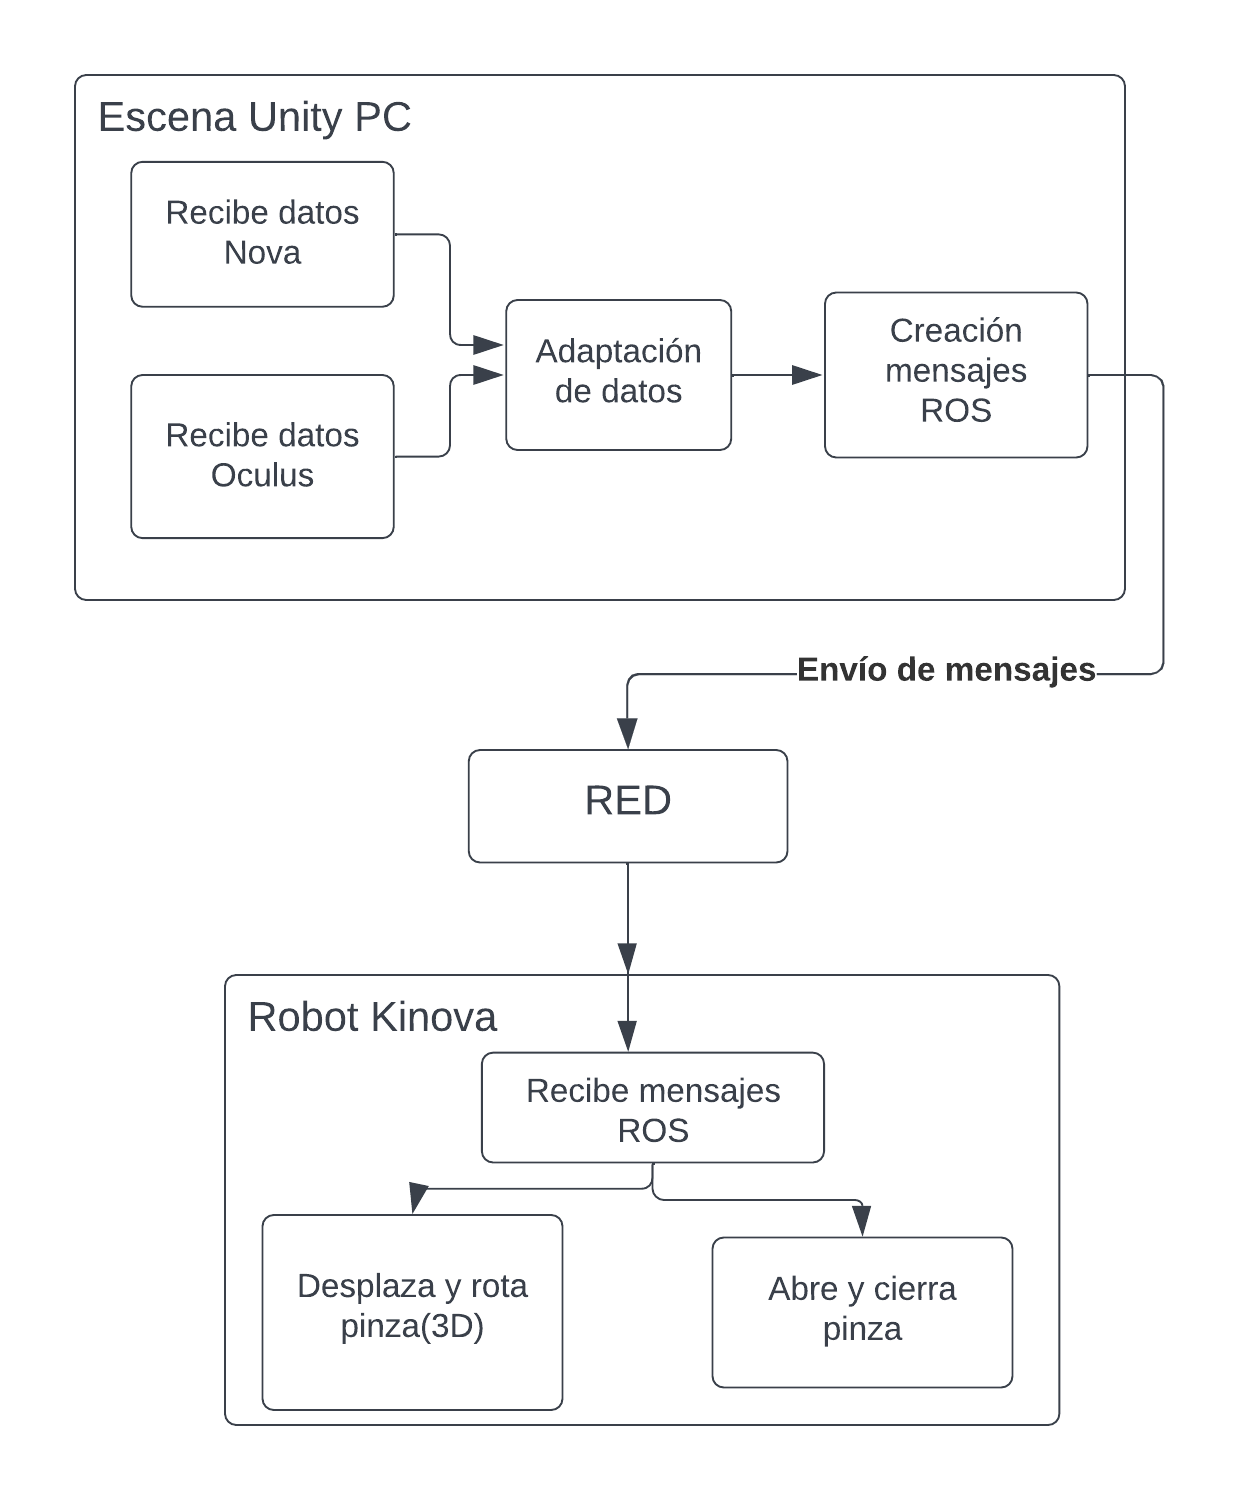
\includegraphics[width=0.9\textwidth]{img/diagrama arquitectura.png}
\caption{Diagrama de la arquitectura del software final}
\end{figure}


